\section{Auswertung}
\label{sec:Auswertung}

Die Materialeigenschaften der auf der Grundplatte verbauten Stäbe werden der Versuchsdurchführung entnommen und in Tabelle \ref{tab:1} angegeben.

\begin{table}
  \centering
  \caption{Materialeigenschaften der Grundplatte. \cite{sample}}
  \label{tab:1}
  \sisetup{table-format=1.2}
  \begin{tabular}{c c c c c c}
    \toprule
    {$\text{Material}$} & {$l \:/\: \si{\centi\metre}$} & {$b \:/\: \si{\centi\metre}$} & {$h \:/\: \si{\centi\metre}$} & {$\rho \:/\: \si{\kilo\gram\per\metre\tothe{3}}$} & {$c \:/\: \si{\joule\per\kilo\gram\per\kelvin} $} \\
    \midrule
    Messing  & 9 & 1.2 & 0.4 & 8520 & 385 \\
    Messing  & 9 & 0.9 & 0.4 & 8520 & 385 \\
    Aluminium  & 9 & 1.2 & 0.4 & 2800 & 830 \\
    Edelstahl  & 9 & 1.2 & 0.4 & 8000 & 400 \\

    \bottomrule
  \end{tabular}
\end{table}

Zunächst wird die erste Messung, wie in Kapitel \ref{sec:stat} beschrieben, durchgeführt.
In Abbildung \ref{fig:1} wird der zeitliche Verlauf für $T_1$ und $T_4$ dargestellt, in \ref{fig:2} der zeitliche Verlauf von $T_5$ und $T_8$.

\begin{figure}
  \centering
  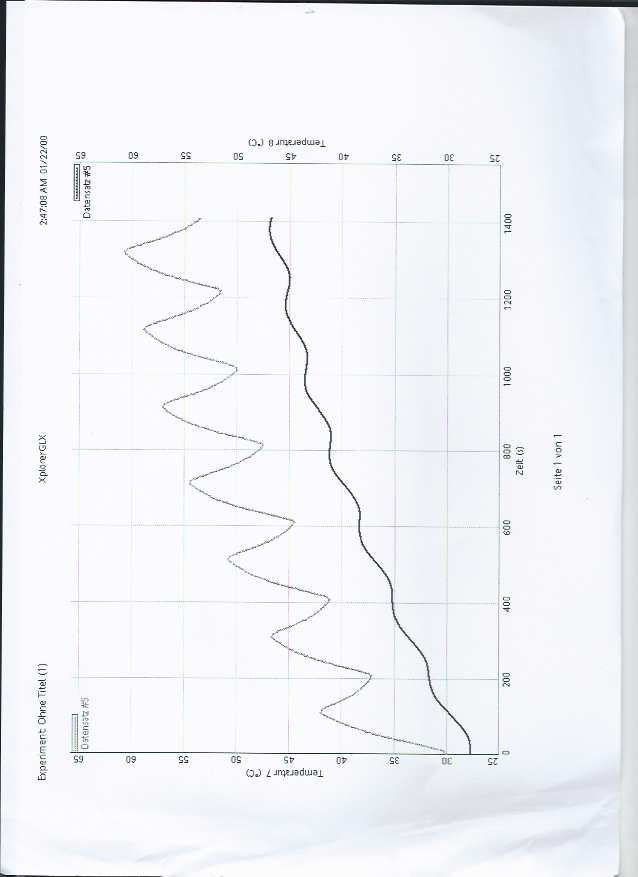
\includegraphics[height=13cm, angle=90]{scan-7.jpg}
  \caption{Zeitlicher Temperaturverlauf von $T_1$ und $T_4$.}
  \label{fig:1}
\end{figure}

\begin{figure}
  \centering
  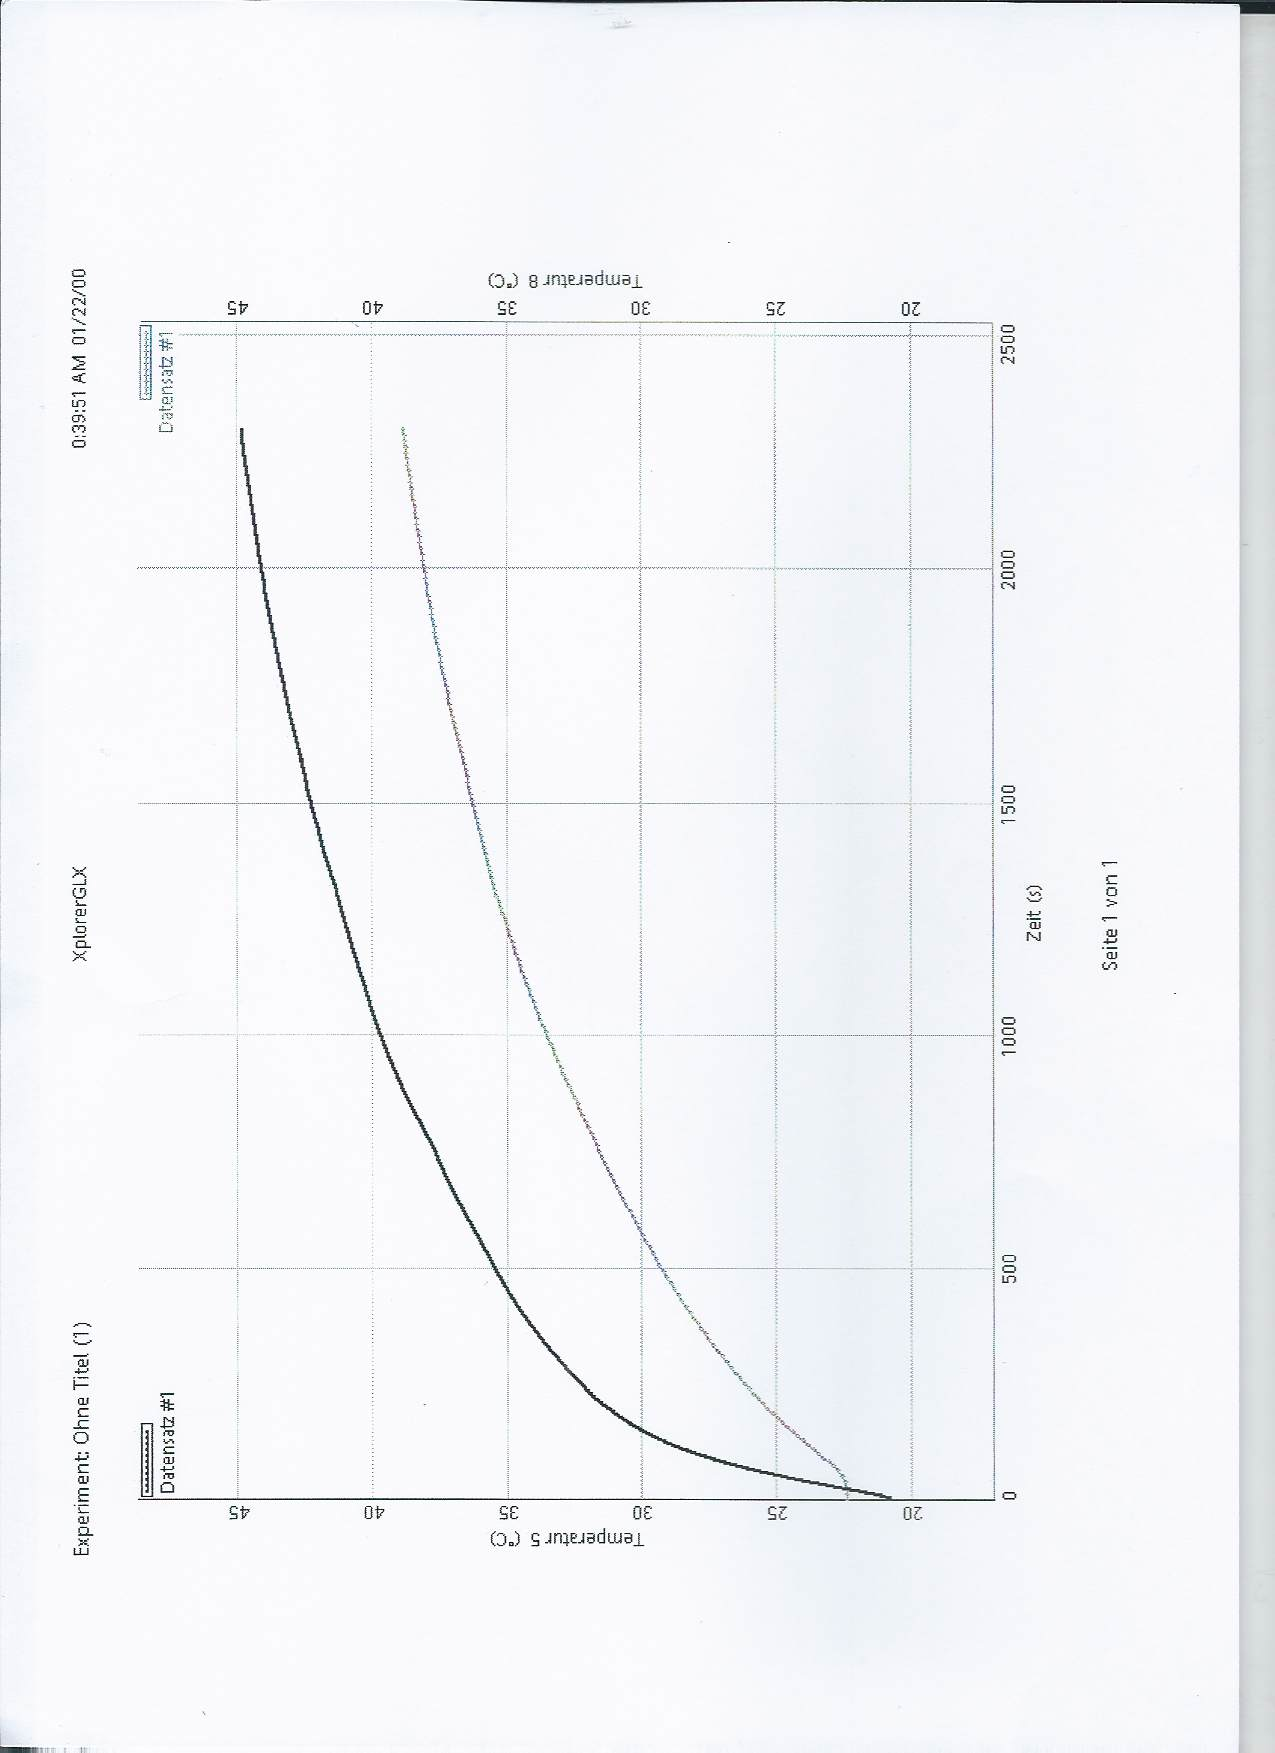
\includegraphics[height=13cm, angle=90]{scan-6.jpg}
  \caption{Zeitlicher Temperaturverlauf von $T_5$ und $T_8$.}
  \label{fig:2}
\end{figure}

Für Abbildung \ref{fig:1} fällt auf, dass beide Graphen eine ähnliche Form aufweisen.
Nach ca. $\SI{200}{\second}$ bildet sich eine Temperaturdifferenz, die nach ungefähr $\SI{500}{\second}$ konstant $\SI{1}{\kelvin}$ beträgt.
Die Graphen wachsen bis zum Ende der Messung in einer identischen Form weiter.
Diese Ähnlichkeiten lassen sich darauf zurückführen, dass es sich um das gleiche Material, nämlich Messing handelt.
Die Unterschiede werden durch die Unterschiedlichen Ausmaße verursacht.\\
Für Abbildung \ref{fig:2} fällt auf, dass der Graph von $T_5$ eine zu Beginn stärkere Steigung aufweist als der Graph von $T_8$.
Nach einiger Zeit stellt sich eine annähernd konstante Temperaturdifferenz von ca. $\SI{6}{\kelvin}$ ein, welche bis zum Ende der Messung besetehen bleibt.
Grund hierfür ist, dass es sich einerseits um Aluminium handelt, welches scheinbar eine bessere Wärmeleitfähigkeit als das andere Material, nämlich Edelstahl, besitzt.\\
Betrachtet man genauer die Temperaturen, welche für die verschiedenen Messpunkte nach $\SI{700}{\second}$ auftreten, so erhält man
\begin{align*}
  T_1 &= \SI{35.70}{\celsius}, \\
  T_4 &= \SI{34.73}{\celsius}, \\
  T_5 &= \SI{37.26}{\celsius}, \\
  T_8 &= \SI{31.14}{\celsius}. \\
\end{align*}
Diese Werte führen zu der Annahme, dass die beste Wärmeleitfähigkeit bei Aluminium vorliegt, gefolgt von Messing, wobei hier die Wärmeleitfähigkeit von den Maßen abhängt.
Die geringste Wärmeleitfähigkeit kann dem Edelstahl zugeordnet werden.\\
Der Wärmestrom, der zu einem bestimmten Zeitpunkt fließt, kann nach Gleichung \ref{eqn:w} berechnet werden.
Es werden dafür die Temperaturen $T_1$ und $T_2$, also von Messing betrachtet.
Die Temperaturdifferenzen können der Abbildung \ref{fig:3} entnommen werden, die weiteren Größen sind
\begin{align*}
  \increment{x} &= \input{build/x_ws.tex}\si{\metre} \\
  A &= \input{build/a_ws.tex}\si{\metre\tothe{3}} \\
  \kappa_\text{Messing} &= \input{build/k_ws.tex}\si{\watt\per\metre\per\kelvin} \\
\end{align*}
wobei $\increment{x}$, der Abstand der Messstellen, am Aufbau abgelesen wird, der Querschnitt $A$ aus Tabelle \ref{tab:1} errechnet und $\kappa_\text{Messing}$ der Literatur entnommen wird.
Es ergeben sich somit die in Tabelle \ref{tab:2} angegebenen Wärmeströme für die jeweligen Messzeiten.

\begin{table}
  \centering
  \caption{Wärmeströme für Messing.}
  \label{tab:2}
  \sisetup{table-format=1.2}
  \begin{tabular}{c c}
    \toprule
    {$t \:/\: \si{\second}$} & {$\frac{\increment{Q}}{\increment{t}} \:/\: \si{\watt}$}\\
    \midrule
    \input{build/wstrom.tex}
    \bottomrule
  \end{tabular}
\end{table}


\begin{figure}
  \centering
  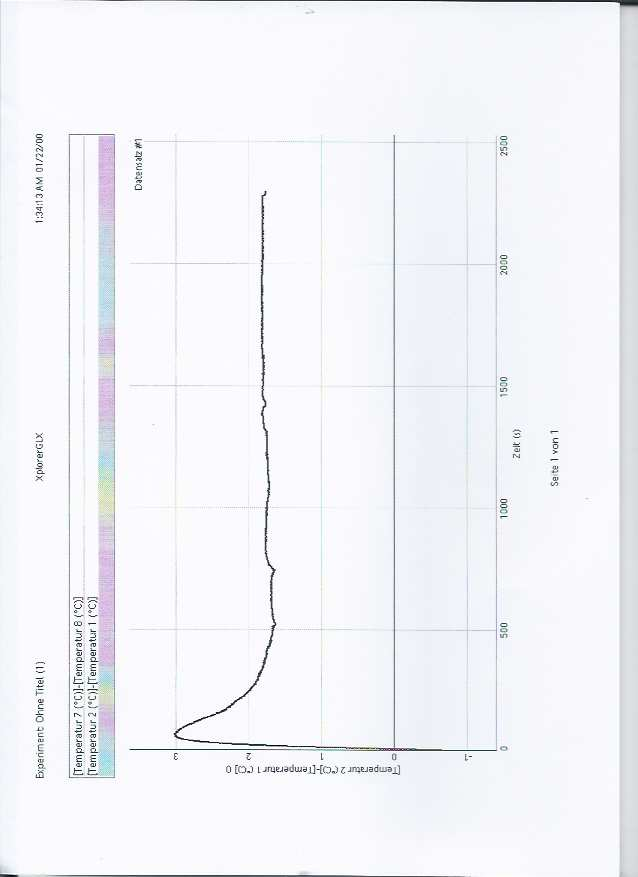
\includegraphics[height=13cm, angle=90]{scan-4.jpg}
  \caption{Zeitlicher Verlauf der Temperaturdifferenz von $T_2$ zu $T_1$.}
  \label{fig:3}
\end{figure}

\begin{figure}
  \centering
  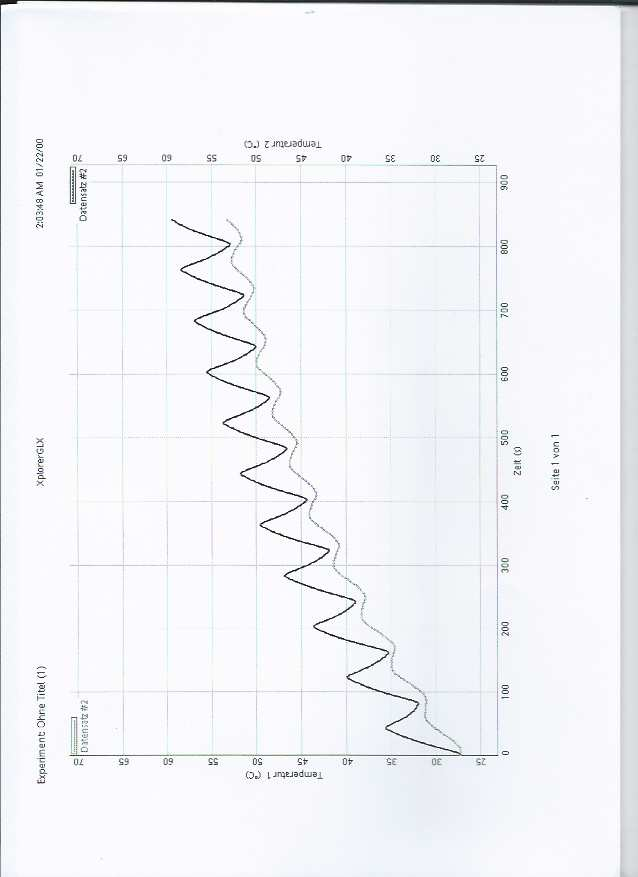
\includegraphics[height=13cm, angle=90]{scan-5.jpg}
  \caption{Zeitlicher Verlauf der Temperaturdifferenz von $T_7$ zu $T_8$.}
  \label{fig:4}
\end{figure}


%\begin{table}
%  \centering
%  \caption{Beispieltabelle}
%  \label{tab:tabelle_beispiel}
%  \sisetup{table-format=1.2}
%  \begin{tabular}{c c}
%    \toprule
%    {$a [\si{\second}]$} & {$b [\si{\kelvin}]$}\\
%    \midrule
%    1.0000  & 11.00 \\
2.0000  & 12.00 \\
3.0000  & 13.00 \\
4.0000  & 14.00 \\
5.0000  & 15.00 \\
6.0000  & 16.00 \\
7.0000  & 17.00 \\
8.0000  & 18.00 \\
9.0000  & 19.00 \\
10.0000 & 20.00 \\

%    \bottomrule
%  \end{tabular}
%\end{table}
%
%Es ergibt sich
%\begin{align}
%  a &= (0 \pm 0) ~ \si{\joule\per\kelvin\per\gram}
 \\
%\end{align}
